
\chapter[AM generation and Demodulation using AD 633]{AM generation and Demodulation using AD 633}
\section*{Aim}
To design and implement AM generation and demodulation using multiplier IC AD633.
\section*{Theory}
DSB-SC using AD633 has already been discussed in chapter \ref{chapdsbsc}. DSB-SC is same as AM devoid of the carrier. Inorder to obtain the complete AM waveform which is \emph{double side band with carrier}, add the carrier signal to the DSB-SC signal. This can be done using the 633 multiplier IC. For more details on IC, refer \ref{AD633}.
\begin{equation}
W= \frac{X.Y}{10}+Z
\end{equation}
\begin{equation}
W= \frac{Emsin(2\pi f_mt).Ecsin(2\pi f_ct)}{10}+E_c sin(2\pi f_ct)
\end{equation}
\begin{equation}
W= \frac{E_mE_c [cos (2\pi (f_c\ -\ f_m)t)]}{20}- \frac{E_mE_c[cos (2\pi (f_c\ +\ f_m)t)]}{20}+E_c sin(2\pi f_ct)
\end{equation}

\paragraph{}
	The resultant AM can be demodulated in two ways,
 \begin{enumerate}

\item
Using Diode envelope detector.
\item
Using another AD633 in cascade with AM generating circuit for multiplying the AM with the carrier.
\end{enumerate}

Multiplying the AM with the carrier once again will result in the following output.
\begin{equation}
\begin{split}
W=\frac{1}{10} &[ \frac{E_mE_c [cos (2\pi (f_c\ -\ f_m)t)]}{20}- \frac{E_mE_c[cos (2\pi (f_c\ +\ f_m)t)]}{20}\\
&\quad +E_c sin(2\pi f_ct)].E_c sin(2\pi f_ct)
\end{split}
\end{equation}

\begin{equation}
\begin{split}
W=& \frac{{E_c}^2}{20}+\frac{E_m.{E_c}^2}{200}sin(2\pi f_mt) \\
&\quad -\frac{{E_c}^2}{20}cos(2\pi(2f_m)t) \\
&\quad +\frac{E_m.{E_c}^2}{400}sin(2\pi (2f_c-f_m)t)  -  \frac{E_m.{E_c}^2}{400}sin(2\pi (2f_c+f_m)t)
\end{split}
\end{equation}

Thus the signal consists of various frequencies of which, the smallest is the message frequency. It can be extracted by filtering using a low pass filter. Since the amplitude of the message frequency is very small, It may be amplified using a simple non-inverting amplifier using an opamp.

\section*{Design}
Provide the supply voltage of +15 V to pin 8 of the IC and -15 V to pin 5 of the IC.\\

\noindent To the \textbf{Y} and \textbf{Z} inputs of the IC, feed the carrier sinusoid of amplitude $E_c=2.5\ V$ and frequency $f_c= 100\ kHz$.\\
To the \textbf{X} input of the IC, feed the message sinusoid of amplitude $E_m=2.5\ V$ and frequency $f_m= 1\ kHz$.\\

\noindent The output AM signal will have a waveform as given by,

\begin{equation}
W=\frac{X.Y}{10}+Z
\end{equation}
\begin{equation}
W=\frac{e_m.e_c}{10}+e_c
\end{equation}
\begin{equation}
W=\frac{6.25}{20}[cos 2\pi 99kt-cos 2\pi 101kt]+2.5 sin(2\pi100kt)
\end{equation}

\noindent Thus it contains two sidebands and the carrier, ie \emph{Double sideband - Full Carrier AM}.
\paragraph{Demodulation:}
Detection may be done using a diode envelope detector as already discussed in chapter \ref{agcdetect}.

An alternate method of demodulation is by multiplying the AM signal once again with the carrier. This can be implemented by connecting another AD633 IC in cascade with the first one.

\noindent The multiplication will result in the following output, as per the theory already explained.

\begin{equation}
\begin{split}
W=& \frac{6.25}{20} +\frac{15.625}{200}sin(2\pi 1kt)\\
&\quad  -\frac{6.25}{20}cos(2\pi 2kt) +\frac{15.625}{400}sin(2\pi199kt) -\frac{15.625}{400}sin(2\pi 201kt)
\end{split}
\end{equation}

\noindent This waveform is shown in Figure \ref{AM633plot2}, which is the stage -1 in demodulation. The next step is to obtain the message signal. This is done by lowpass filtering the above signal at a cut-off frequency of 1.5 kHz.

To design an RC lowpass filter of cut-off frequency 1.5 kHz,

\begin{equation}
f_c=\frac{1}{2\pi R_1C_1}=1.5kHz
\end{equation}
Choose $C_1=0.01\  \mu F$
$\therefore  R_1 =10 \ k \Omega$

A non-inverting amplifier may be used to amplify this signal. Using a feedback resistor of $R_f= 100 \ k \Omega$ and an input resistance of $R_i=10\ k\Omega$ will result in a gain of $A_v=1+\frac{R_f}{R_i}=11$.
\section*{Circuit Diagram}
The circuit diagram for generating AM(DSB-FC) and demodulating it using AD633 multiplier IC as shown in Figure. \ref{633amckt}. 

\begin{sidewaysfigure}[ht]
    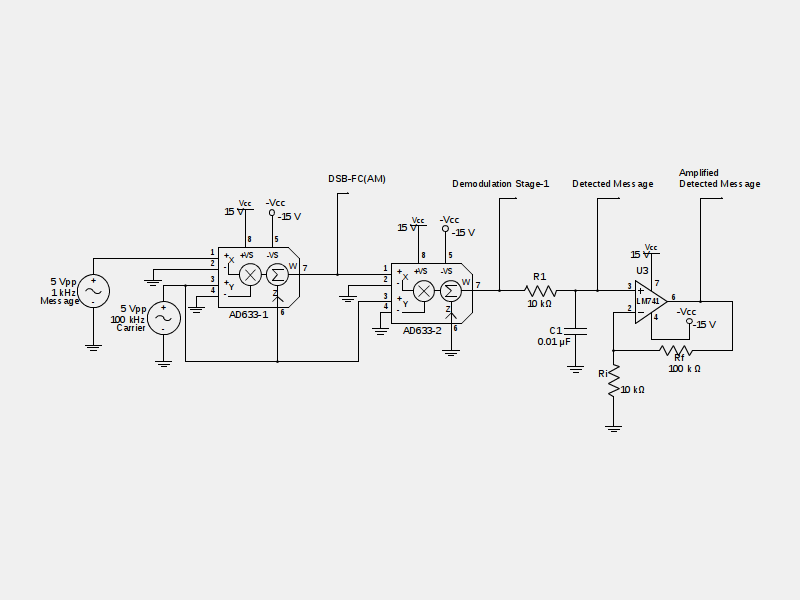
\includegraphics[scale=0.8, trim=0cm 4cm 0cm 4cm,clip=true]{633amckt.png}
    \caption{Circuit for AM generation and detection using AD633 multiplier IC}
    \label{633amckt}
\end{sidewaysfigure}


\section*{Procedure}
\begin{itemize}
\item
Make connections as shown in the circuit diagram, figure \ref{633amckt}.
\item
Feed the message and carrier signals.
\item
Connect the pin number 7 of the first IC to a CRO and observe the resultant waveform which is AM(DSB-FC).
\item
Connect the pin number 7 of the second IC to a CRO and observe the resultant waveform which is the product of DSB-FC and the carrier.(Named demodulation stage-1 signal)
\item
Observe the output from the filter, amplified by the opamp amplifier, which extracts the envelope of the signal-\emph{The 1kHz message signal}.
\item
Plot the signals observed on a graph sheet.
\end{itemize}
\section*{Observation}
The input and output signals as observed on a CRO are shown in Figure \ref{AM633plot1}and \ref{AM633plot2}.
\begin{figure}[ht]
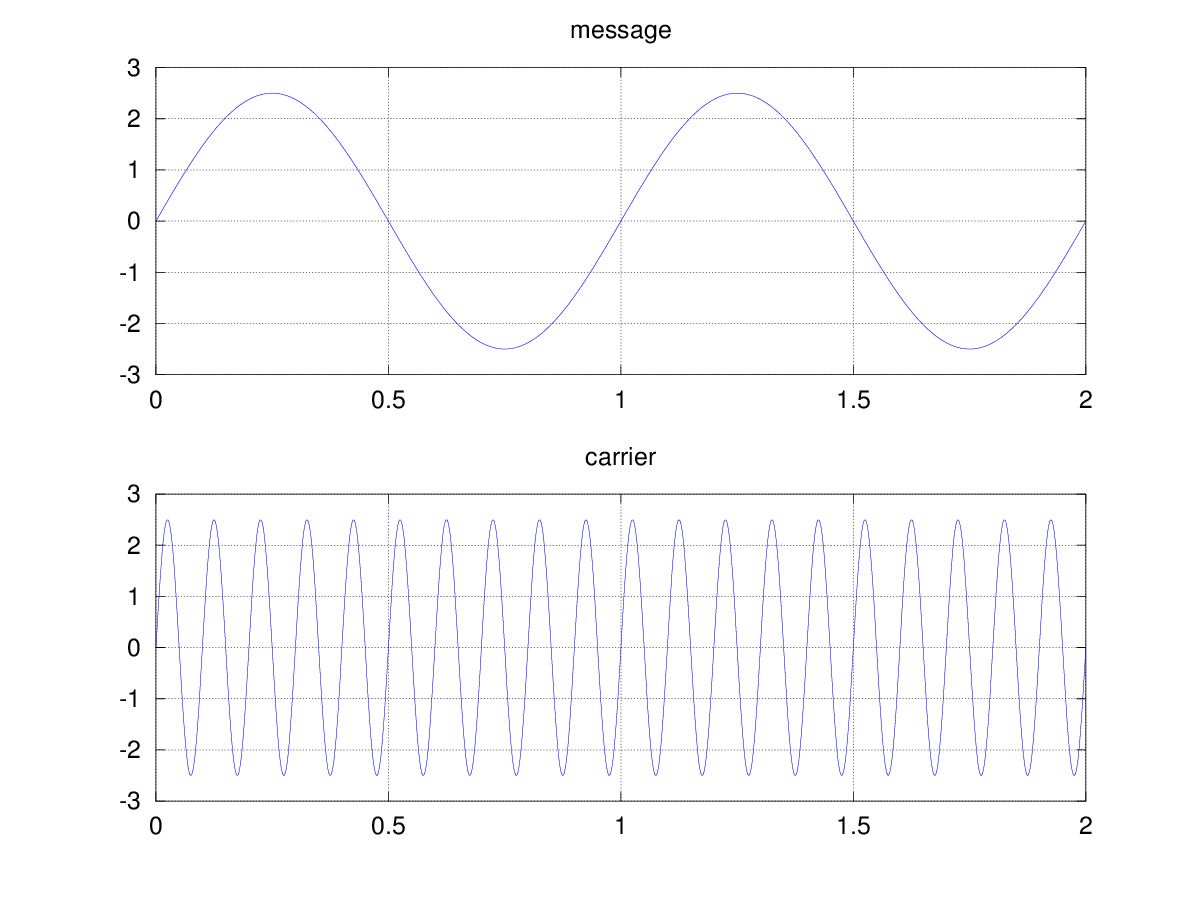
\includegraphics[width=\textwidth]{am6331.png}
\caption{Message and carrier signals}
\label{AM633plot1}
\end{figure}

\begin{figure}[ht]
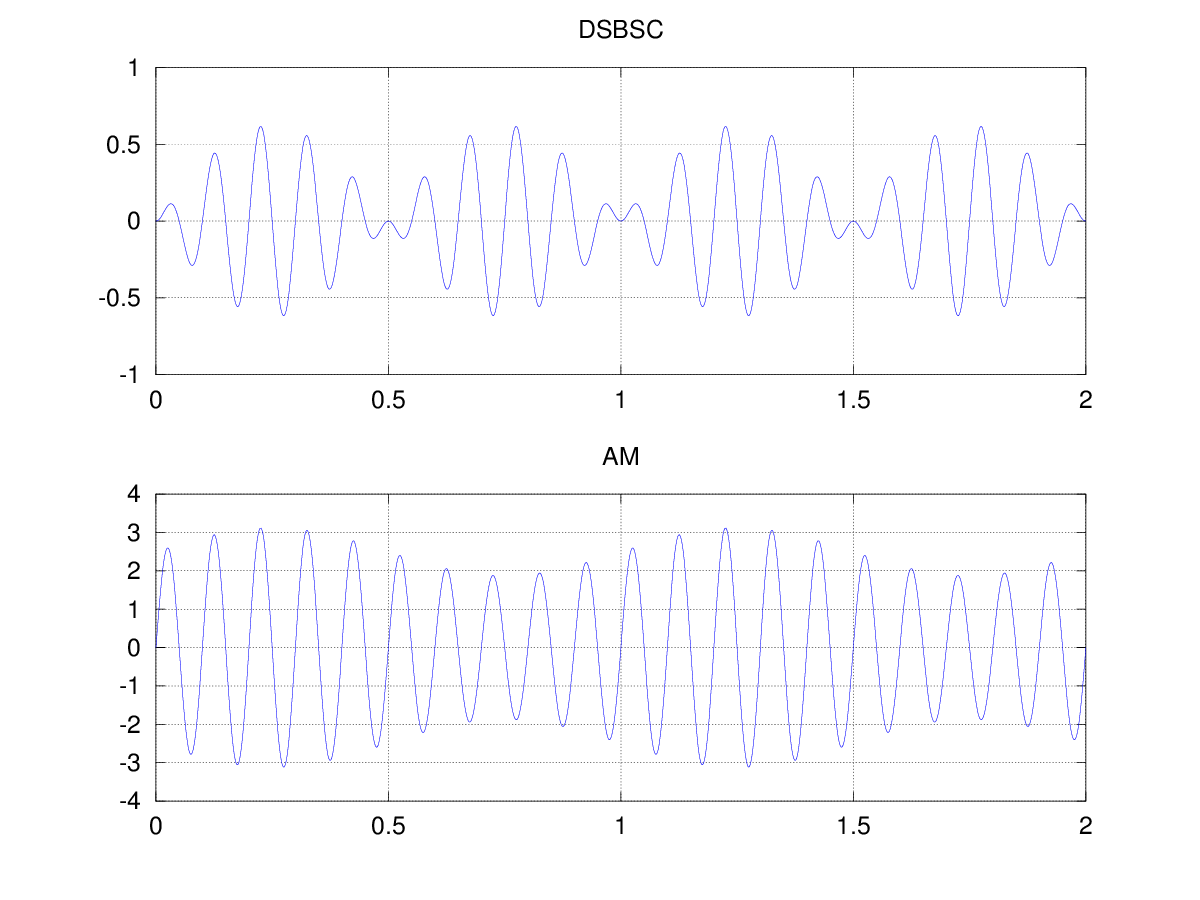
\includegraphics[width=\textwidth]{am6332.png}
\caption{AM(DSB-FC) and Demodulation stage-1 signals}
\label{AM633plot2}
\end{figure}


\section*{Result}
Implented the AM generation and demodulation circuit using multiplier IC and opamps.
The resultant waveforms were plotted.